\documentclass[12pt]{article}
\usepackage[top=1in,left=1in, right = 1in, footskip=1in]{geometry}

\usepackage{graphicx}
%\usepackage{adjustbox}

%% \newcommand{\comment}{\showcomment}
\newcommand{\comment}{\nocomment}

\newcommand{\showcomment}[3]{\textcolor{#1}{\textbf{[#2: }\textsl{#3}\textbf{]}}}
\newcommand{\nocomment}[3]{}

\newcommand{\jd}[1]{\comment{cyan}{JD}{#1}}
\newcommand{\swp}[1]{\comment{magenta}{SWP}{#1}}

\newcommand{\eref}[1]{Eq.~\ref{eq:#1}}
\newcommand{\fref}[1]{Fig.~\ref{fig:#1}}
\newcommand{\Fref}[1]{Fig.~\ref{fig:#1}}
\newcommand{\sref}[1]{Sec.~\ref{#1}}
\newcommand{\frange}[2]{Fig.~\ref{fig:#1}--\ref{fig:#2}}
\newcommand{\tref}[1]{Table~\ref{tab:#1}}
\newcommand{\tlab}[1]{\label{tab:#1}}
\newcommand{\seminar}{SE\mbox{$^m$}I\mbox{$^n$}R}

\usepackage{amsthm}
\usepackage{amsmath}
\usepackage{amssymb}
\usepackage{amsfonts}

% \usepackage{lineno}
% \linenumbers

\usepackage[pdfencoding=auto, psdextra]{hyperref}

\usepackage{natbib}
\bibliographystyle{chicago}
\date{\today}

\usepackage{xspace}
\newcommand*{\ie}{i.e.\@\xspace}

\usepackage{color}

\newcommand{\Rx}[1]{\ensuremath{{\mathcal R}_{#1}}} 
\newcommand{\Ro}{\Rx{0}}
\newcommand{\RR}{\ensuremath{{\mathcal R}}}
\newcommand{\Rhat}{\ensuremath{{\hat\RR}}}
\newcommand{\tsub}[2]{#1_{{\textrm{\tiny #2}}}}

\begin{document}

\begin{flushleft}{
	\Large
	\textbf\newline{
		Unraveling the paradox between generation and serial intervals: applications to COVID-19 pandemic
	}
}
\newline\\
Sang Woo Park
\end{flushleft}

\section*{Abstract}

\pagebreak

%The key distributions for understanding the spread of COVID-19 include:
%\begin{enumerate}
%  \item Incubation period distribution: time between infection and symptom onset \citep{backer2020incubation, %li2020early, linton2020incubation, tian2020characteristics}
%  \item Serial interval distribution: time between symptom onset of an infector and an infectee \citep{du2020s%erial, nishiura2020serial, zhao2020estimating}
%  \item Generation interval distribution: time between infection of an infector and an infectee \citep{ganyani%2020estimating}
%\end{enumerate}

\section{Introduction}

Since the emergence of the novel coronavirus disease (COVID-19), a significant amount of research has focused on estimating its reproduction number $\mathcal R$ \citep{majumder2020early}.
The reproduction number is defined as the average number of secondary cases caused by a primary case;
the corresponding reproduction number in a fully susceptible population --- referred to as the basic reproduction number $\mathcal R_0$ --- allows us to predict the extent to which a disease will spread in the population and the amount of intervention to prevent an outbreak \citep{anderson1991infectious}.
Since the reproduction number cannot be measured directly, it is often estimated from the observed exponential growth rate using generation- and serial-interval distributions.

The generation interval is defined as the time between when an individual (infector) is infected and when an individual infects another person (infectee);
the generation-interval distributions plays a key role in shaping the relationship between the exponential growth rate $r$ and the reproduction number $\mathcal R$.
On the other hand, the serial interval is defined as the time between when an infector and an infectee become symptomatic.
While serial intervals are similar to generation intervals, previous studies noted that using serial intervals can give different estimates of $\mathcal R$ and have often alluded to differences in their variances, despite having seemingly identical expected values.
Even though these distinctions were first made over a decade ago \citep{svensson2007note}, 
the need for a better conceptual and theoretical framework for understanding their differences is becoming clearer as the COVID-19 pandemic unfolds:
Researchers continue to rely on both generation and serial intervals to estimate $\mathcal R$ for COVID-19 without making a clear distinction.

The lack of clear understanding of their differences can be largely attributed to an apparent paradox.
When the epidemic is growing exponentially, the spread of infection can be characterized as a ``renewal process'' based on previous incidence of infection, the associated generation-interval distribution, and the average infectiousness of an infected individual.
This renewal formulation allows us to link the exponential growth rate of an epidemic $r$ with its reproduction number $\mathcal R$.
Likewise, since infection typically leads to symptoms, we should be able to describe the renewal process of symptomatic cases using the serial-interval distribution.
Therefore, both generation- and serial-interval distributions should give us identical estimates of  $\mathcal R$ based the observed epidemic growth rate $r$.
However, current theory suggests that using generation- and serial-interval distributions give different estimates of $\mathcal R$ and contradicts our biological intution.

Here, we provide an answer to the decade-old paradox between generation and serial intervals.
We present a novel framework for understanding serial intervals and show that the serial-interval distribution must be defined with reference to disease incidence;
previous frameworks implicitly assume that incidence remains constant.
Using our framework, we are able to show that both serial- and generation-interval distributions give identical estimates of $\mathcal R$ based on the exponential growth phase of an epidemic.
However, failing to account for changes in the observed serial-interval distributions over time can severely bias the estimate of $\mathcal R$.
We apply our framework to serial intervals of COVID-19 and lay out several principles to consider in using information about serial intervals and other epidemiological time delays in the analysis of the ongoing pandemic.

\section{Methods}

\subsection{Backward and forward delay distributions}

We first begin by describing a general framework for characterizing a distribution of time delays between \emph{any} two epidemiological events;
these events can be defined either within an infected individual (e.g., infection and symptom onset of an individual) or between infected individuals (e.g., symptom onsets of an infector and an infectee).
We can further divide these events into \emph{primary} and \emph{secondary} events.
When we measure an epidemiological time delay within an infected individual (e.g., incubation period), the primary event always occurs before the secondary event.
When we measure an epidemiological time delay between infected individuals (e.g., serial interval), 
the primary and secondary events are defined in terms of the direction of transmission:
The primary event refers to the event that occurs within an infector and does not necessarily occur before the secondary event.

We model time delays between a primary and a secondary event from a cohort perspective.
A primary cohort consists of \emph{all} individuals whose primary event occurred at a given time; 
a secondary cohort can be defined similarly based on the secondary events.
For example, when we are measurign serial intervals, a primary cohort $s$ consists of all infectors who became symptomatic at time $s$.
Then, for each primary cohort $s$, we can define the expected time distribution between primary and secondary events.
We refer to this distribution as the forward delay distribution and denote it as $f_s(\tau)$.
The forward delay distributions can vary across primary cohorts.

Likewise, we can define the backward delay distribution $b_s(\tau)$ for a secondary cohort $s$:
The backward delay distribution for secondary host $s$ describes the time delays between a primary and secondary host given that the secondary event occurred at time $s$.
It follows that:
\begin{equation}
b_s(\tau) \propto C(s-\tau) f_{s-\tau}(\tau)
\end{equation}
where $C(s)$ is the size of the primary cohort $s$.
Therefore, changes in the backward delay distribution depends on the changes in cohort size $C(s)$ (therefore incidence of infection) as well as changes in the forward delay distribution.
These ideas apply to all epidemiological delay distributions and generalize the work by \citep{champredon2015intrinsic} who compared forward and backward generation-interval distributions to describe the realized generation intervals from the perspective of an infector and an infectee, respectively.

\subsection{Realized serial interval distributions}

The serial interval is defined as the time between when an infector becomes symptomatic and when and infectee becomes symptomatic.
Serial intervals $\tau$ are typically written as:
\begin{equation}
\tau = - x_0 + \sigma + x_1
\end{equation}
where $x_0$ and $x_1$ represent the realized time from infection to symptom onset of an infector and an infectee, respectively, and $\sigma$ represents the realized generation interval.
Previous studies have often assumed that $x_0$ and $x_1$ have the same means and concluded that the serial and generation intervals have the same mean;
however, these results implicitly assume that incidence stays constant.

\begin{figure}[!th]
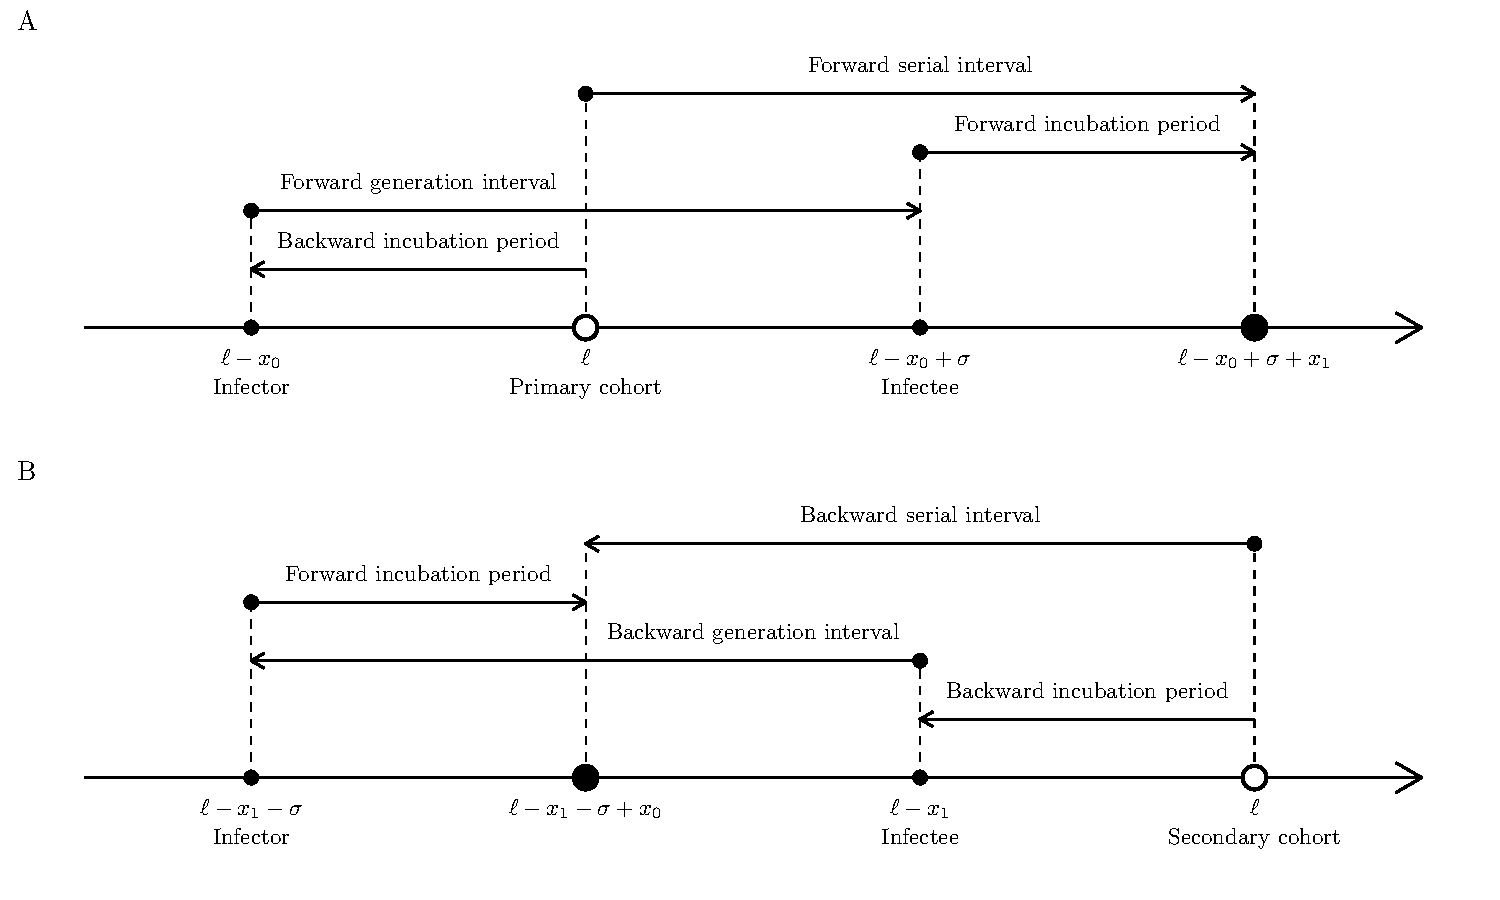
\includegraphics[width=\textwidth]{serial_guide.pdf}
\caption{
\textbf{Forward and backward serial intervals.}
}
\label{fig:diagram}
\end{figure}

Using the cohort-based framework provides a clear way of understanding the serial-interval distribution.
Given that an infector became symptomatic at time $\ell$, we have to first go backward in time by asking when the infector was infected and go forward in time by asking when the infector infected infectee and when the infectee became symptomatic;
this defines the forward serial interval (\fref{diagram}A).
Then, it is clear that $x_0$ represents the backward incubation period of infectors who became symptomatic at time $\ell$; 
$\sigma$ represents the forward generation interval for individuals who came infected at time $\ell - x_0$ conditional on their incubation period $x_0$;
and $x_1$ represents the forward incubation period for the infectees who became infected at time $\ell - x_0 + \sigma$.
Assuming that the forward incubation distribution does not vary across cohorts, the forward serial interval distribution of a primary cohort $\ell$ can be written as follows:
\begin{equation}
f_\ell(\tau) \propto \int_{0}^\infty \int_{0}^\infty \mathcal R_c (\ell - x_0) i(\ell - x_0) h_{\ell - x_0}(x_0, \sigma) k(\tau-\sigma+x_0) \mathrm{d} x_0\, \mathrm{d}\sigma
\end{equation}
where $i$ is the incidence of infection, $h$ is the joint probability distribution of the forward incubation period and forward generation interval of a primary cohort $\ell - x_0$, and $k$ is a marginal probability distribution of $h$ describing the forward incubation periods:
\begin{equation}
k(x_0) = \int_0^\infty h_\ell(x_0, \sigma) \mathrm{d}\sigma.
\end{equation}
Finally, $\mathcal R_c (\ell - x_0)$ is the cohort reproduction number, which is defined as the average secondary number of cases caused by an individual infected at time $\ell - x_0$.
We have to multiply the joint forward distribution $h$ by $\mathcal R_c (t) i(t)$, which represents total infectiousness of individuals infected at time $t$, rather than incidence $i(t)$, because we are interested in the backward incubation period $x_0$ and the forward generation interval $\sigma$ of infectors, rather than all infected individuals.
We revisit this idea in the Results section.

Likewise, we can define the backward serial interval distribution for a secondary cohort $\ell$ (\fref{diagram}B).
Given that an infectee became symptomatic at time $\ell$, we have to first go backward in time by asking when the infectee became infected and when the infector became infected; 
then, we have to go forward in time by asking when the infector became symptomatic.
In this case, $x_1$ and $\sigma$ represent the backward incubation period and generation interval, respectively, and $x_0$ represents the forward incubation period.
Therefore, the backward serial interval distribution of a secondary cohort $\ell$ can be written as follows
\begin{equation}
\begin{aligned}
b_\ell(\tau) &\propto j(\ell) f_{\ell}(\tau)\\
&\propto \int_0^\infty i(\ell-x_0) k(x_0) f_{\ell}(\tau) \mathrm{d} x_0
\end{aligned}
\end{equation}
where $j$ represents the incidence of symptomatic cases.

\subsection{Epidemic model}

Here, use a renewal equation to model the spread of disease in a population:
\begin{equation}
i(t) = \mathcal R_0 S(t) \int_0^\infty i(t-\tau) g(\tau) \mathrm{d}\tau,
\label{eq:renewal}
\end{equation}
where $\mathcal R_0$ is the basic reproduction number (i.e., the average number of secondary cases caused by a primary case  in a fully susceptible population), $g(\tau)$ is the intrinsic generation-interval distribution (i.e., the forward generation-interval distribution of a primary case in a fully susceptible population), $S(t)$ is the proportion of susceptible individuals.
Then, the forward generation-interval for a primary cohort $\ell$ follows \citep{champredon2015intrinsic}:
\begin{equation}
g_\ell (\tau) \propto g(\tau) S(\ell + \tau),
\end{equation}
which allows us to separate the joint probability distribution $h_\ell$ of the forward incubation period and the forward generation-interval distribution as a product of joint probability distribution $h$ of the forward incubation period and the intrinsic generation intervals and the proportion of susceptible individuals $S$:
\begin{equation}
h_\ell (x_0, \tau) \propto h(x_0, \tau) S(\ell + \tau),
\end{equation}
which satisfies the following:
\begin{equation}
g(\tau) = \int_0^\infty h(x_0, \tau) \mathrm{d}x_0.
\end{equation}
Finally, the cohort reproduction is defined as follows:
\begin{equation}
\mathcal R_c(t) = \mathcal R_0 \int_0^\infty g(\tau) S(t+\tau) \mathrm{d} \tau.
\end{equation}

\subsection{Linking $r$ and $\mathcal R$}

During the initial phase of an epidemic, the proprotion susceptible remains constant ($S(t) = S(0)$) and incidence of infection grows exponentially: $i(t)=i_0\exp(rt)$.
Then, we can estimate the reproduction number from the exponential growth rate $r$ via the Euler-Lotka equation:
\begin{equation}
\frac{1}{\mathcal R} = \int_0^\infty \exp(-r\tau) g(\tau) \mathrm{d} \tau.
\end{equation}
Like forward generation-interval distributions, 
forward serial-interval distributions describe the renewal process of symptomatic cases.
Therefore, the forward serial-interval distribution $f_{\textrm{\tiny exp}}(\tau)$ during the exponential growth phase provides the identical $r$--$\mathcal R$ link as the intrinsic generation-interval distribution:
\begin{equation}
\frac{1}{\mathcal R} = \int_{-\infty}^\infty \exp(-r\tau) f_{\textrm{\tiny exp}}(\tau) \mathrm{d} \tau,
\end{equation}
where the forward serial-interval distribution during the exponential growth phase is defined as:
\begin{equation}
f_{\textrm{\tiny exp}}(\tau) \propto \int_{0}^\infty \int_{0}^\infty \exp( -r x_0) h(x_0, \sigma) k(\tau-\sigma+x_0) \mathrm{d} x_0\, \mathrm{d}\sigma.
\end{equation}
In Appendix, we provide a mathematical proof that this relationship holds.

We note that the forward serial-interval distribution depends on the exponential growth rate $r$.
When the epidemic grows fast (high $r$), we expect the backward incubation period to be short, and therefore, the forward serial-interval distribution will generally have a larger mean than the intrinsic generation-interval distribution.
The Susceptible-Exposed-Infected-Recovered model, which assumes that incubation and exposed periods are equivalent, is a special case where the conditional forward generation-interval distribution cancels out with the backward generation-interval distribution exactly because (i) infected individuals can only transmit after symptom onset and (ii) the time between symptom onset to infection is independent of the incubation period of an infector;
in this case, the forward serial- and generation-intervals have the same distributions during the exponential growth phase.

\begin{table}[!th]
\begin{center}
\begin{tabular}{|l|l|r|}
\hline
Parameter & Values & Source\\
\hline
Mean forward incubation period & 5.5 days & \cite{lauer2020incubation} \\
SD forward incubation period & 2.4 & \cite{lauer2020incubation} \\
Mean intrinsic generation interval & 5 days & \cite{ferretti2020quantifying} \\
SD intrinsic generation interval & 2 & \cite{ferretti2020quantifying} \\
\hline
\end{tabular}
\end{center}
\caption{
\textbf{Parameter values used for simulations.}
The intrinsic generation-interval distribution is parameterized using a log-normal distribution with log mean $\mu_G=1.54$ and log standard deviation $\sigma_G=0.37$.
The forward incubation period distribution is parameterized using a log-normal distribution with log mean $\mu_I=1.62$ and log standard deviation $\sigma_I=0.42$.
The joint probability distribution is modeled using a multivariate log-normal distribution with correlations $\rho=-0.5, 0, 0.5$.
}
\end{table}

We use a simulation-based approach to compare the estimates of $\mathcal R$ based on the serial- and generation-interval distributions. 
To do so, we model the intrinsic generation-interval distribution and the incubation period using a multivariate log-normal distribution with log means $\mu_G, \mu_I$, log standard variances $\sigma_G^2, \sigma_I^2$, and correlation $\rho$;
the multivariate log-normal distribution is parameterized based on pameter estimates for COVID-19 (Table 1).
We construct forward serial intervals during the exponential growth period as follows:
\begin{equation}
S_i = -B_i + (G_i|B_i) + I_i,
\end{equation}
where the backward incubation period $B_i$ of an infector is simulated by drawing random log-normal samples $A_i$ with log mean $\mu_I$ and log variance $\sigma_I^2$ and resampling $A_i$, each weighted by the inverse of the exponential growth function $\exp(-rA_i)$;
the intrinsic generation interval conditional on the incubation period of the infector $(G_i|B_i)$ is drawn from a log-normal distribution with log mean $\mu_G + \sigma_G \rho (\log(B_i) - \mu_I)/\sigma_I$ and log variance $\sigma_G^2 (1-\rho^2)$;
the forward incubation period $I_i$ of an infectee is drawn from a log-normal distribution with log mean $\mu_I$ and log variance $\sigma_I^2$.
We then calculate the reproduction number $\mathcal R$ using the empirical estimator:
\begin{equation}
\mathcal R = \frac{1}{\frac{1}{N}\sum_{i=1}^N \exp(- r S_i)}.
\end{equation}
We compare this estimate with a naive estimate of ${\mathcal R}_{\textrm{\tiny naive}}$ that assumes that the backward and the forward incubation periods are identically distributed:
\begin{equation}
{\mathcal R}_{\textrm{\tiny naive}} = \frac{1}{\frac{1}{N}\sum_{i=1}^N \exp(- r T_i)},
\end{equation}
where
\begin{equation}
T_i = -A_i + (G_i|A_i) + I_i.
\end{equation}

\section{Results}

First, we compare the estimates of the reproduction number $\mathcal R$ based on the intrinsic generation-interval distribution and the forward serial-interval distribution during the exponential growth phase (\fref{rR}A).
Both distributions provide identical estimates of $\mathcal R$ regardless of the correlation $\rho$ between the incubation period distribution and the intrinsic generation-interval distribution.
On the other hand, using naive serial-interval distributions that do not account for disease dynamics (i.e., assuming that the backward and the forward incubation period distributions are identical) underestimates $\mathcal R$;
as $r$ increases, ${\mathcal R}_{\textrm{\tiny naive}}$ saturates and eventually decreases due to negative serial intervals (\fref{rR}B).
While the forward serial intervals during the exponential growth phase can be also negative, the proportion of negative intervals are appropriately balanced because faster epidemic growth will lead to shorter backward incubation period (and therefore less negative serial intervals).

\begin{figure}[!th]
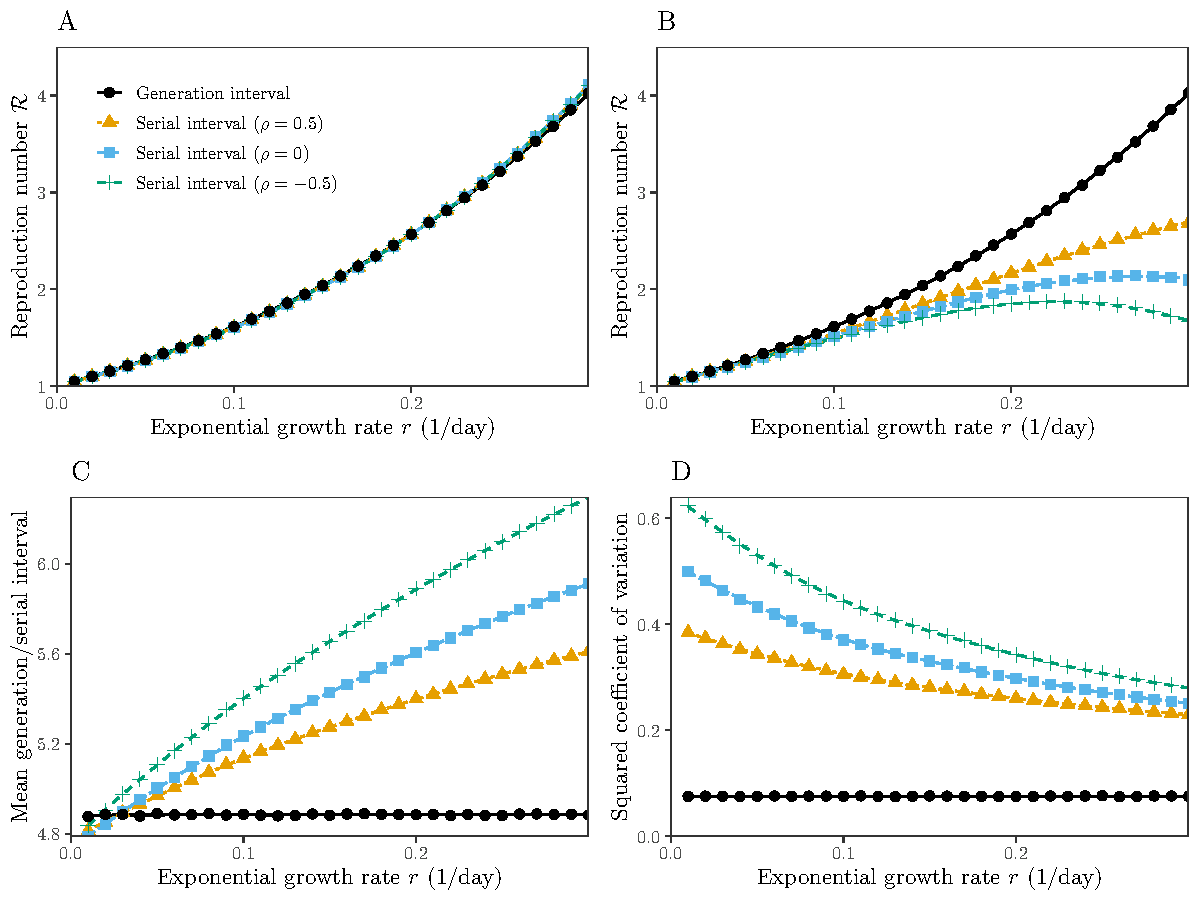
\includegraphics[width=\textwidth]{rR.pdf}
\caption{
\textbf{Estimates of the reproduction number from the exponential growth rate.}
}
\label{fig:rR}
\end{figure}

Comapring the shapes of forward serial-interval distributions and the intrinsic generation-interval distribution allow us to better understand how they are able to give identical estimates of $\mathcal R$.
In general, generation-interval distributions with higher means and less variability are expected to give higher $\mathcal R$ for a given $r$.
In this case, the forward serial intervals during the exponential growth phase have higher means (\fref{rR}C) and squared coefficients of variation (\fref{rR}D) than the intrinsic generation-interval distribution.
The effects of higher means (which increases $\mathcal R$) and higher variability (which decreases $\mathcal R$) cancel out exactly;
therefore, we estimate the same $\mathcal R$ using both serial and generation intervals.

\begin{figure}[!th]
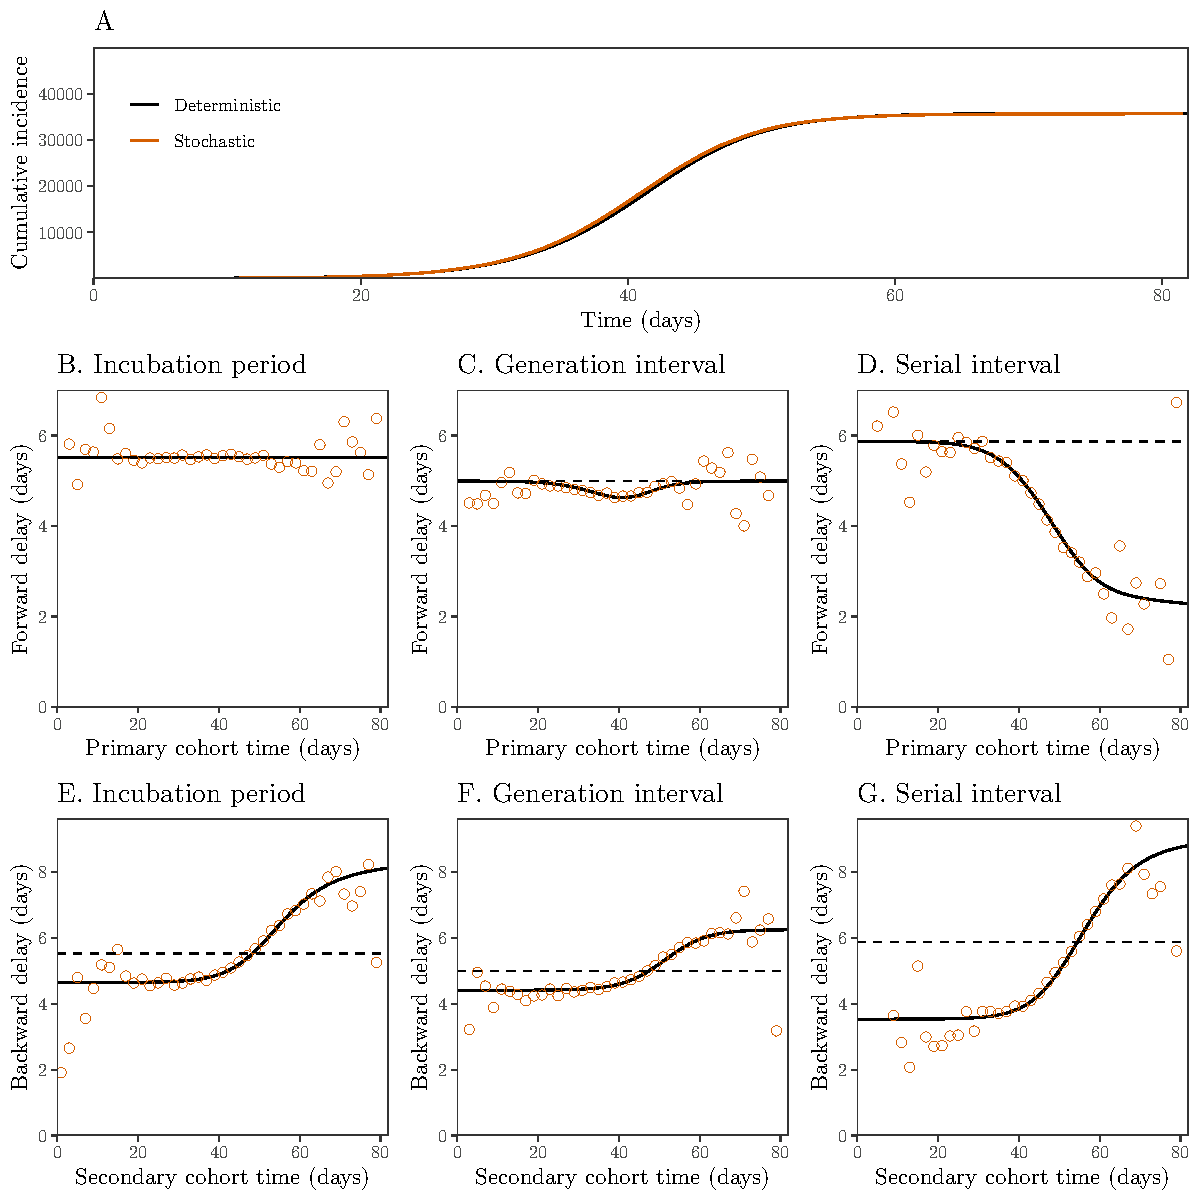
\includegraphics[width=\textwidth]{forward.pdf}
\caption{
\textbf{Epidemiological dynamics and changes in mean forward and backward delay distributions.}
}
\label{fig:epi}
\end{figure}

\fref{epi} compares the epidemiological dynamics (A) with the mean forward (B--D) and the mean backward (E--F) delay distributions of a deterministic model based on the renewal equation (\eref{renewal}) and the corresponding stochastic realization based on the Gillespie algorithm.
The mean forward incubation period remains constant throughout an epidemic as expected (\fref{epi}B).
The mean forward generation interval contracts as the epidemic progresses because an infected individual is less likely to infect another person as the proportion of susceptible individuals decreases (\fref{epi}C; \cite{champredon2015intrinsic}).
In contrast, the mean serial interval depends on previous incidence and therefore decreases over time (\fref{epi}D):
When incidence is increasing, symptomatic individuals are more likely to have been infected more recently (shorter backward incubation period and therefore longer forward serial interval) whereas when incidence is decreasing, symptomatic individuals are more likely to have been infected later (longer backward incubation period and therefore shorter forward serial interval).
Qualitative patterns in the changes in the mean backward delays is robust across all delay distributions because they are predominantly driven by the changes in incidence (\fref{epi}D).

\begin{figure}[!th]
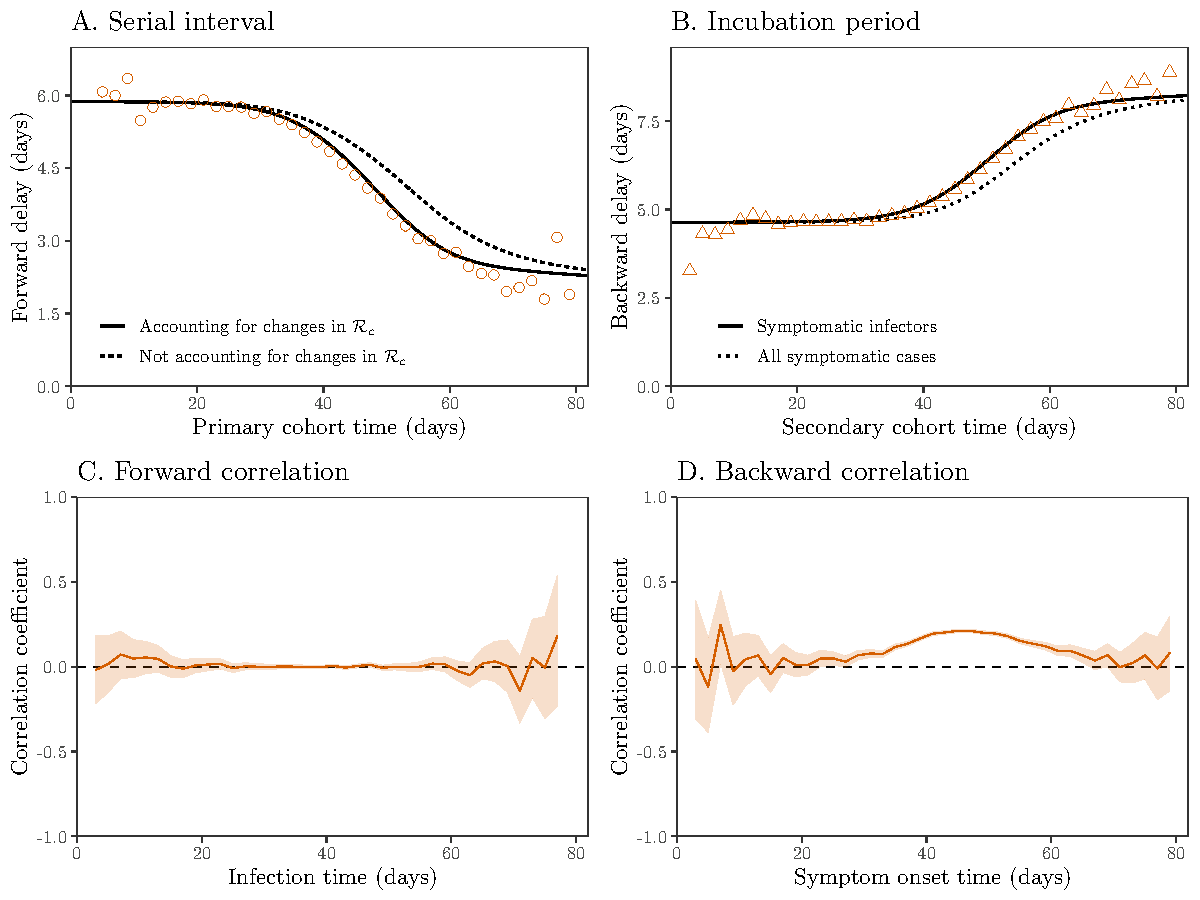
\includegraphics[width=\textwidth]{forward_tease.pdf}
\caption{
\textbf{Effects of dynamical correlations on serial intervals.}
}
\label{fig:tease}
\end{figure}

We further tease apart factors that affect the forward serial interval distribution, including the cohort reproduction number $\mathcal R_c$, as mentioned earlier.
\fref{tease}A compares the mean forward serial interval calculated from a stochastic model (orange points) with their deterministically calculated values;
failing to account for changes in $\mathcal R_c$ overestimates the mean forward serial interval.
A key distinction that needs to be made is that the forward serial-interval distributions depends on the backward incubation period of infectors (i.e., those who were able to successfully spread the disease to another person), rather than the incubation period of all symptomatic cases (\fref{tease}B).
Therefore, the cohort size of infectors must be calculated as a product of the cohort reproduction number and incidence.

Comparing the backward incubation period of infectors and all symptomatic cases provides an important, but counterintuitive, insight (\fref{tease}B).
Given a cohort of symptomatic cases, individuals who were able to successfully spread the disease to others have longer incubation periods, on average;
individuals with longer incubation period are infected earlier and have a higher chance of infecting others (i.e., higher $\mathcal R_c$) during the susceptible depletion phase.
Therefore, the backward incubation period of an infector and the number of secondary cases caused by that infector are dynamically correlated (\fref{tease}C).
This correlation disappears when we take the forward perspective, demonstrating the importance of perspective-dependency in studying epidemiological delay distributions (\fref{tease}D).

\begin{figure}[!th]
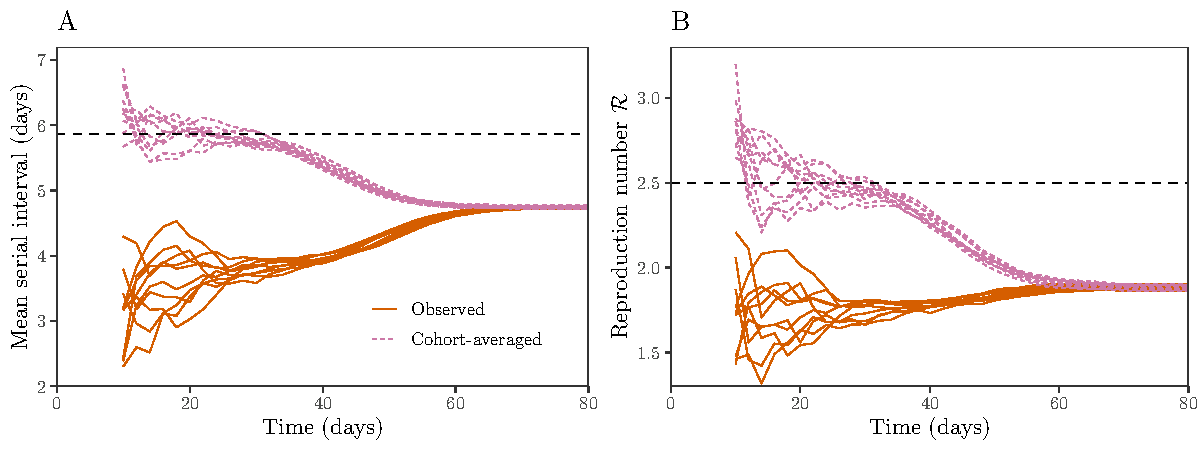
\includegraphics[width=\textwidth]{observedrR.pdf}
\caption{
\textbf{Estimates of the reproduction number from the observed serial intervals.}
}
\label{fig:obsrR}
\end{figure}

Now, we turn to practical issues.
When an epidemic is ongoing, the observed serial intervals are subject to right-censoring because we cannot observe a serial interval if either an infector or an infectee has not yet developed symptoms.
\fref{obsrR} demonstrates how the effect of right-censoring in the observed serial intervals translates to the underestimation of $\mathcal R$.
Notably, even if we can observe \emph{all} serial intervals across all transmission pairs after the epidemic has ended, we still underestimate $\mathcal R$ by a large amount because the observed serial-interval distribution does not account for changes in the forward serial-interval distribution.
As the mean forward serial-interval distribution decreases over time, taking the average of all observed serial intervals throughout an epidemic will underestimate the mean forward serial-interval distribution during the exponential growth phase, which provides the correct linke between $r$ and $\mathcal R$.

We provide a simple, heuristic way of assessing potential biases in the estimate of $\mathcal R$ retrospctively.
Once a set of serial intervals has been observed, we can group observed serial intervals by their primary cohort times.
Then, we can compare how estimates of $\mathcal R$ change as we include more cohorts into the analysis (see `cohort-averaged' in \fref{obsrR}).
During the exponential growth phase, the estimates of $\mathcal R$ are consistent with the true value;
adding more data allows us to make more precise inference about $\mathcal R$ during this period.
However, the cohort-averaged estimates of $\mathcal R$ decreases rapidly soon after the exponential growth period.
Confidence intervals associated with the cohort-averaged estimates of $\mathcal R$ becomes narrower and do not overlap with earlier estimates.
This approach allows us to detect how changes in the forward serial intervals bias the estimates of $\mathcal R$.

\begin{figure}[!th]
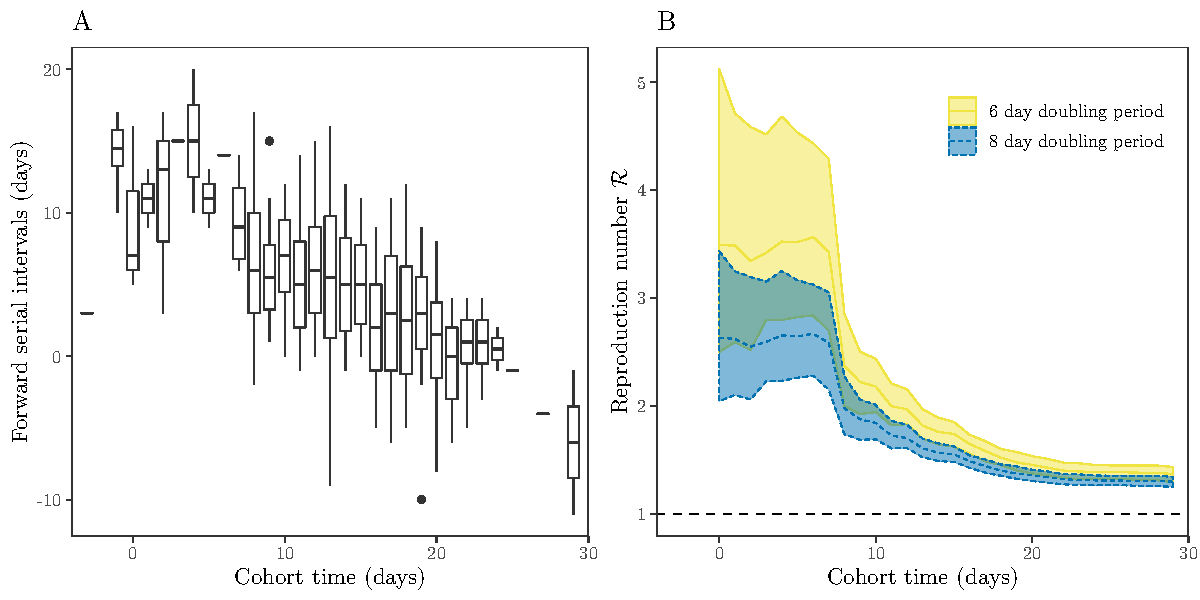
\includegraphics[width=\textwidth]{serial_analysis.pdf}
\caption{
\textbf{Observed serial intervals of COVID-19 and estimates of $\mathcal R$.}
}
\label{fig:du}
\end{figure}

Finally, we revisit serial intervals of COVID-19 collected by \cite{du2020serial} from mainland China, outside Hubei province, based on transmission events reported between January 21--February 8, 2020;
they estimated the mean serial of 3.96 days (95\% CI 3.53–4.39 days) and $\mathcal R_0$ of 1.32 (95\% CI 1.16–1.48).
\fref{du}A shows changes in the forward serial-interval distribution across cohorts.
While the observed serial intervals may be subject to right-censoring, increase in the proportion of negative serial intervals are clearly indicative of the changes in the forward serial-interval distribution.
\fref{du}B shows the cohort-averaged estimates of $\mathcal R_0$, which remain constant until day 7 and suddenly decreases.
The early cohort-averaged estimates are also consistent with earlier estimates.
This example clearly demonstrates the danger of naively averaging the observed serial intervals and calculating the reproduction number from them.

\section{Discussion}

Characterizing generation- and serial-interval distributions are critical to understanding the outset of an outbreak as they determine the time scale of disease transmission.
Generation intervals measure the time difference between infection of a transmission pair, whereas serial intervals measure the time difference between symptom onset of a transmission pair.
Due to their similar definitions, there differences have been inaccurately captured and misunderstood.
Here, we provide a theoretical basis for understanding serial intervals.

First, we demonstrate the importance of defining a cohort for studying any epidemiological time delay distributions.
Previous studies have shown that generation interval can be either measured forward or backward;
we generalize their ideas and show that these ideas can be applied to all distributions.
Changes in the backward delay distributions is particularly robust across all distributions because they depend on previous changes in cohort sizes, which, in turn, depend on incidence of infection.
Several epidemic analyses have attempted to reconstruct symptom onset or infection dates for each case from the confirmed dates while assuming a constant delay distribution;
these assumptions translate to assuming a constant backward delay distribution.
Although such assumption may be able to approximately match the time scale of an epidemic, 
our analysis reveals that it is not a safe assumption.

Using cohort-based approaches, we define forward and backward serial intervals.
The forward serial-interval distribution describes the renewal process of the symptomatic cases and therefore provides the correct link between $r$ and $\mathcal R$.
While our results support the use of serial interval distributions for calculating $\mathcal R$, 
they also reveal gaps in our current understanding and practical approaches to characterizing serial intervals.


\pagebreak

\section*{Appendix}

Recall that the forward serial interval can be written as:
\begin{equation}
- x_0 + \sigma + x_1
\end{equation}
Note that $x_1$ is independent of $x_0$ and $\sigma$. Then, we get:
\begin{equation}
M_{- x_0 + \sigma + x_1}(-r) = M_{- x_0 + \sigma}(-r) M_{x_1}(-r).
\end{equation}
We want to show that 
\begin{equation}
M_{- x_0 + \sigma}(-r)= \frac{M_\sigma(-r)}{M_{x_1}(-r)}
\end{equation}
for $r \geq 0$.
Note that the time between symptom onset and infection of an infectee follows the following distribution:
\begin{equation}
z(\tau) \propto \int_{\max(0, -\tau)}^\infty i(\ell - x_0) h_{\ell - x_0}(x_0, \tau+x_0) \mathrm{d} x_0.
\end{equation}
During the exponential growth phase, we have
\begin{equation}
\begin{aligned}
z_{\textrm{\tiny exp}}(\tau) &= \frac{1}{N} \int_{\max(0, -\tau)}^\infty \exp(- r x_0) h(x_0, \tau+x_0) \mathrm{d} x_0\\
% &= \frac{1}{N} \int_{0}^\infty \left[ \exp(- r x_0) k(x_0) \times \frac{h(x_0, \tau+x_0)}{k(x_0)}\right] \mathrm{d} x_0
\end{aligned}
\end{equation}
where $N$ is the normalization factor:
\begin{equation}
\begin{aligned}
N &= \int_{-\infty}^\infty \int_{\max(0, -\tau)}^\infty \exp(- r x_0) h(x_0, \tau+x_0) \mathrm{d} x_0\,\mathrm{d}\tau\\
&= \int_{0}^\infty \int_{-x_0}^\infty \exp(- r x_0) h(x_0, \tau+x_0) \mathrm{d}\tau\,\mathrm{d} x_0\\
&= \int_{0}^\infty \exp(- r x_0) k(x_0) dx_0\\
&= M_{x_1}(-r)
\end{aligned}
\end{equation}
Therefore,
\begin{equation}
\begin{aligned}
&\int_{-\infty}^{\infty} \exp(-r\tau) z_{\textrm{\tiny exp}}(\tau) \mathrm{d}\tau\\
&=\frac{1}{M_{-x_1}(-r)} \int_{-\infty}^{\infty} \exp(-r\tau) \int_{\max(0, -\tau)}^\infty \exp(- r x_0) h(x_0, \tau+x_0) \mathrm{d} x_0\, \mathrm{d}\tau
\end{aligned}
\end{equation}

Finally, we are left to prove that 
\begin{equation}
\int_0^{\infty} \exp(-r\tau) g(\tau) \mathrm{d}\tau = \int_{-\infty}^{\infty} \exp(-r\tau) \int_{\max(0, -\tau)}^\infty \exp(- r x_0) h(x_0, \tau+x_0) \mathrm{d} x_0\, \mathrm{d}\tau
\end{equation}
where $g$ is a marginal probability distribution of $h$ describing the forward generation intervals:
\begin{equation}
g(\tau) = \int_0^\infty h(x_0, \tau)  \mathrm{d} x_0.
\end{equation}
Let $a = x_0 + \tau$. Then, by change of variables, it immediately follows that
\begin{equation}
\begin{aligned}
&\int_{-\infty}^{\infty} \exp(-r\tau) \int_{\max(0, -\tau)}^\infty \exp(- r x_0) h(x_0, \tau+x_0) \mathrm{d} x_0\, \mathrm{d}\tau\\
&=\int_{0}^{\infty} \int_{0}^\infty \exp(- r a) h(x_0, a) \mathrm{d} x_0\, \mathrm{d}a\\
&=\int_{0}^{\infty} \exp(-r\tau) g(\tau) \mathrm{d}\tau
\end{aligned}
\end{equation}
Therefore, the forward serial- and generation-interval distributions give the same link between $r$ and $\mathcal R$.

\bibliography{serial}

\end{document}
